\section{Sensors}

A \textbf{sensor} is a device that measures a property of the environment, collecting data that can be either external or internal to the vehicle.
Based on what they measure, sensors are divided into two families: \textbf{exteroceptive} sensors measure the properties of the \textbf{external environment} (e.g.\ radar, LiDAR, cameras), while \textbf{proprioceptive} sensors measure the properties of the \textbf{ego vehicle} itself (e.g.\ wheel encoders, IMU).
The same classification can also be applied to the software that processes their data.

The number and the complexity of the sensors mounted on a vehicle have increased drastically over the past few years, since every new ADAS/AD function requires a better and wider perception of the surroundings.

\begin{figure}[H]
    \centering
    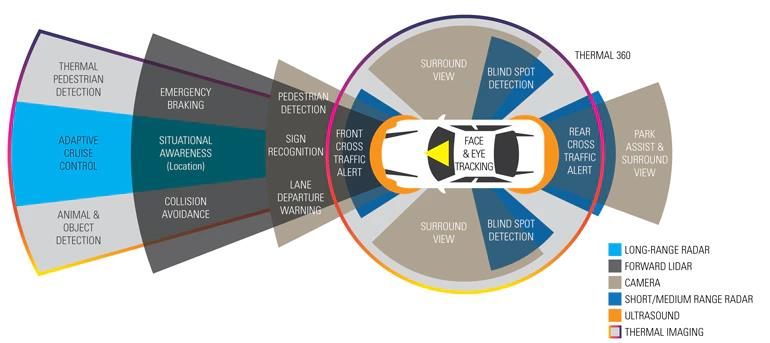
\includegraphics[width=0.6\textwidth]{images/C3_1.png}
    \caption{Sensors around the vehicle and the functions they enable}
\end{figure}

To compare different sensors we look at a set of relevant parameters:

\begin{table}[H]
    \centering
    \begin{tabular}{|p{2.6cm}|p{7cm}|p{6cm}|}
        \hline
        \textbf{Parameter} & \textbf{Definition} & \textbf{Importance} \\
        \hline
        \textbf{Range} & Maximum distance at which the sensor can detect objects (short, middle, long range) & Determines how far a sensor can see \\
        \hline
        \textbf{Field of View (FoV)} & Angular width that the sensor can observe in the horizontal and vertical planes (e.g.\ 360° only horizontally) & A wider FoV covers more area \\
        \hline
        \textbf{Wavelength} & Range of electromagnetic waves used by the sensor (visible light, infrared, radio waves, \dots) & Affects resolution, robustness to weather and performance in different lighting conditions \\
        \hline
        \textbf{Spatial coverage} & Dimensional extent (2D or 3D) of the area captured at any given time & Needed to understand the environment in 3D \\
        \hline
        \textbf{Resolution} & Smallest detail the sensor can distinguish & Higher resolution gives more detailed information about objects \\
        \hline
        \textbf{Update rate} & Frequency at which the sensor captures/refreshes data (Hz) & Higher update rates give more timely information \\
        \hline
        \textbf{Robustness to weather} & Ability of the sensor to work under adverse weather conditions & Robust sensors operate reliably in various conditions \\
        \hline
    \end{tabular}
    \caption{Relevant parameters of the sensors}
\end{table}

\subsection{Ranging sensors}
The first family of sensors we analyse are the \textbf{ranging sensors}: LiDAR, radar and ultrasonic sensors. They are all \textbf{active} sensors: they emit a signal (light, radio waves or sound) and measure the \textbf{distance} of the objects from the time the signal takes to come back (\textbf{time of flight}). What changes is the type of signal, and therefore their resolution, range, cost and robustness to weather.

\subsubsection{LiDAR}
\begin{wrapfigure}{R}{0.41\textwidth}
    \centering
    \vspace{-10pt}
    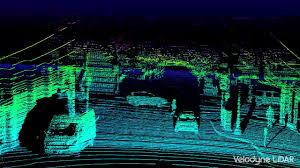
\includegraphics[width=0.4\textwidth]{images/C3_2.png}
    \caption{LiDAR point cloud}
    \vspace{-10pt}
\end{wrapfigure}
\textbf{LiDAR} (Light Detection And Ranging) is a technology used to scan objects and to \textbf{measure distances and reflectivity}.
A pulsed LiDAR transmits \textbf{laser beams} (infrared light) that bounce off the objects and return to the sensor.
It works on the \textbf{time of flight} principle: the distance of an object is computed from how long the pulse takes to travel back, while the \textbf{intensity} is the strength of the returned beam.
For this reason LiDARs struggle with \textbf{black} surfaces, which absorb the light and return a very weak signal.

The output of a LiDAR is a \textbf{point cloud}, a set of 3D points that looks like a shadow of the scene and reflects the shape and size of the objects.
Modern sensors produce millions of points per second (from 1.4 million of a Velodyne HDL-32E up to almost 26 million of a Robosense EM4), and all these points have to be processed in real time.
LiDARs are very \textbf{expensive} and are \textbf{affected by bad weather} (rain, fog, snow).

They are mainly used to build \textbf{high-resolution maps} and to \textbf{localize} the car in a map, but also for \textbf{object detection}.
To detect objects we typically rely on the \textbf{density} of the points: a very dense area is probably an object, but we do \textbf{not} know \textbf{what} kind of object it is.
Neural networks can classify the points, but the results are not great, so the classification is usually done with the help of \textbf{cameras} (computer vision).

\begin{infobox}[Phantom braking]
Many phantom brakings happen because the obstacle detection relies only on the LiDAR: a plastic bag flying in front of the car is detected as a solid object, and the vehicle brakes.
\end{infobox}

\paragraph{Types of LiDAR}
The main distinction is between LiDARs with and without moving parts.

\textbf{Mechanical LiDARs} are the most common type: they use mirrors and a \textbf{rotation motor} to sweep the laser beam over 360°.
Their drawbacks are the high cost of the mechanical parts and their sensitivity to vibrations (e.g.\ when the road is not smooth, like on cobblestones).

\textbf{Solid-state LiDARs} do not require spinning components, so they are resistant to vibrations, compact and cheaper, at the cost of a \textbf{reduced FoV}.
There are two main technologies: \textbf{MEMS} LiDARs use a tiny tilting mirror (Micro-Electro-Mechanical System), driven by electrostatic or magnetic actuators, to scan the laser beam across the scene with a predefined pattern; \textbf{Flash} LiDARs instead project a single broad laser pulse that covers the whole FoV in one shot, and capture the returned 3D data with a time-of-flight sensor array.

\begin{figure}[H]
    \centering
    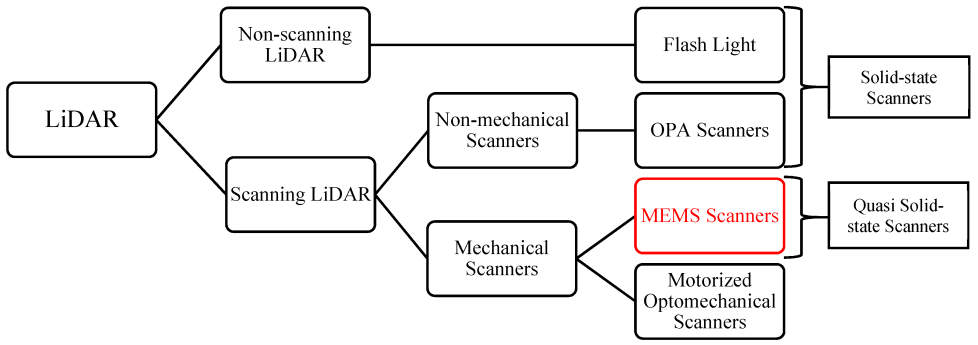
\includegraphics[width=0.5\textwidth]{images/C3_3.png}
    \caption{Classification of the LiDARs}
\end{figure}

LiDARs can also be classified by \textbf{dimensionality}.
A \textbf{1D} LiDAR has a single laser beam that measures the distance along one axis; a \textbf{2D} LiDAR spins one beam to collect the horizontal distances, obtaining data on $X$ and $Y$; a \textbf{3D} LiDAR shoots multiple beams spread along the vertical axis, obtaining data on $X$, $Y$ and $Z$.

\begin{figure}[H]
    \centering
    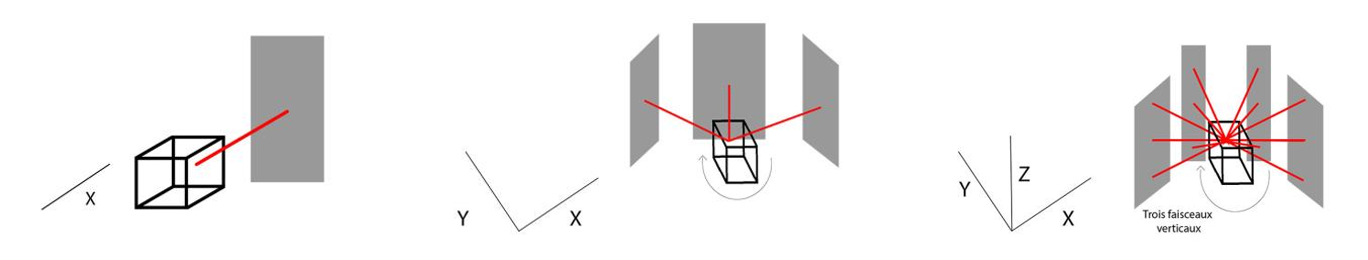
\includegraphics[width=0.8\textwidth]{images/C3_6.png}
    \caption{1D, 2D and 3D LiDAR}
\end{figure}

\paragraph{Multiple return}
With \textbf{multiple return} technology a LiDAR can capture \textbf{several reflections from a single laser pulse}, since the pulse can hit more objects along its path.
For example, the first return may come from a raindrop or from dust, while the following ones come from more distant objects like vehicles, pedestrians or the road.
This allows to see beyond rain, fog or dust clouds.

Some LiDARs (e.g.\ Ouster) let the user choose the packet format: in \textbf{single return} mode only the strongest return of each pulse is captured (as most commercial LiDARs do), while in \textbf{dual return} mode both the strongest and the first return are captured.
To remove the dust we just have to filter out the first return.

\begin{figure}[H]
    \centering
    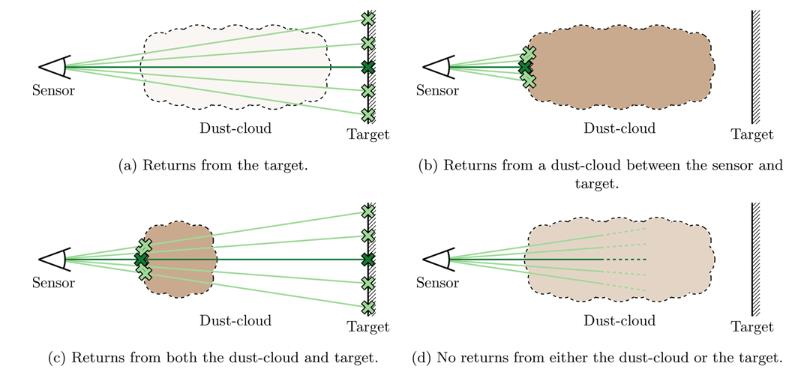
\includegraphics[width=0.55\textwidth]{images/C3_7.png}
    \caption{Returns in presence of a dust cloud}
\end{figure}

\paragraph{Use cases}
LiDARs are used to implement several AD functionalities, each one with its typical algorithms:
\begin{compactitemize}
    \item \textbf{Object detection}: \textit{PointPillars} represents the point cloud as a 2D pseudo-image (pillars) and applies a CNN.
    \item \textbf{Object recognition}: \textit{PointNet} directly processes the raw 3D points and classifies the objects by their geometric shape.
    \item \textbf{Multi-object tracking}: \textit{Kalman Filter/EKF} estimates the future positions of the objects from their current state (position, velocity, \dots).
    \item \textbf{Intention prediction}: \textit{LSTM} networks predict the future trajectories of the objects from their past movements.
    \item \textbf{Localization}: \textit{ICP} (Iterative Closest Point) aligns the point cloud to a reference map or to the previous frames.
\end{compactitemize}

\paragraph{Metrics}
\begin{wrapfigure}{R}{0.36\textwidth}
    \centering
    \vspace{-10pt}
    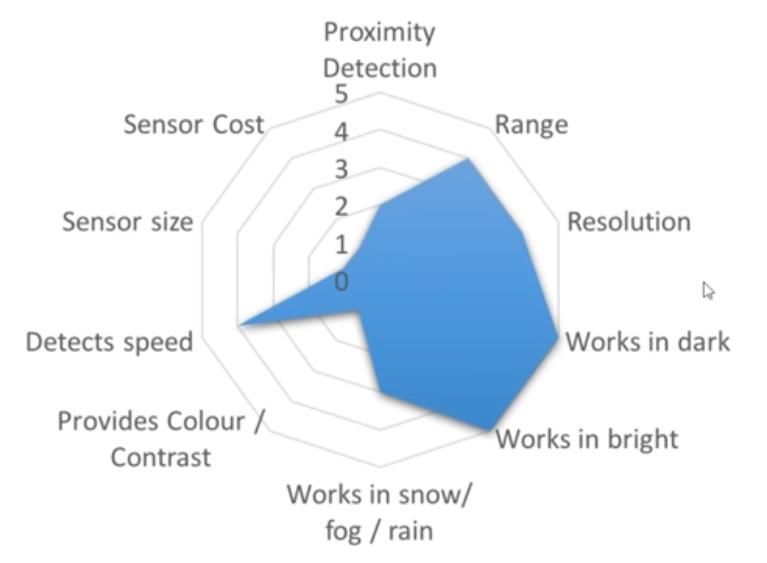
\includegraphics[width=0.35\textwidth]{images/C3_8.png}
    \caption{LiDAR strengths and weaknesses}
    \vspace{-10pt}
\end{wrapfigure}
The most relevant metrics of a LiDAR are the \textbf{number of beams}, the \textbf{points per second} (the more points, the more detailed the map), the \textbf{rotation rate} (Hz), the \textbf{detection range}, the \textbf{field of view}, the \textbf{wavelength} and the \textbf{weather resistance} (IP level).

Summing up, the LiDAR gives extremely accurate depth information, with a resolution much higher than radar and 360° of visibility, and it works both in the dark and in bright light.
On the other hand it is expensive, bulky, it does not measure the speed of the objects directly and it does not provide colour: colour LiDARs do not exist yet, even if they are starting to appear.

\paragraph{Reading LiDAR data}
The sensor sends its data as \textbf{UDP packets}, which are then converted into a point cloud.
Usually a driver is provided, but writing our own driver can be very useful when we need efficiency.

Point clouds are often stored in the \textbf{PCD} (Point Cloud Data) format, whose header describes the cloud: \texttt{FIELDS} gives the name of each dimension of a point, \texttt{SIZE} the size of each dimension in bytes, \texttt{WIDTH} and \texttt{HEIGHT} the number of points (for an organized, image-like cloud of $640\times480$ we have $307200$ points), \texttt{POINTS} the total number of points and \texttt{DATA} the storage type (ascii or binary).

\begin{lstlisting}[language={}]
# .PCD v.7 - Point Cloud Data file format
VERSION .7
FIELDS x y z rgb
SIZE 4 4 4 4
TYPE F F F F
COUNT 1 1 1 1
WIDTH 213
HEIGHT 1
VIEWPOINT 0 0 0 1 0 0 0
POINTS 213
DATA ascii
0.93773 0.33763 0 4.2108e+06
0.90805 0.35641 0 4.2108e+06
...
\end{lstlisting}

\subsubsection{Radar}
\begin{wrapfigure}{r}{0.29\textwidth}
    \centering
    \vspace{-10pt}
    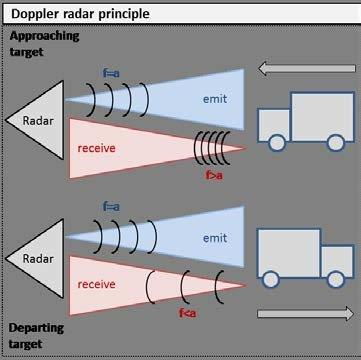
\includegraphics[width=0.28\textwidth]{images/C3_10.png}
    \caption{Doppler effect}
    \vspace{-10pt}
\end{wrapfigure}
\textbf{Radar} (Radio Detection and Ranging) is conceptually similar to the LiDAR, but instead of light beams it uses \textbf{radio waves} to detect the objects and to measure their \textbf{distance}, \textbf{angle} and \textbf{speed} with respect to the ego vehicle.

The \textbf{distance} is computed from the time and frequency difference between the transmitted and the reflected wave.
If the object is moving, the reflected wave comes back with a slight \textbf{frequency shift}, due to the \textbf{Doppler effect}: the frequency increases if the target is approaching and decreases if it is moving away, so the radar can directly measure the \textbf{radial velocity} of the objects.
Finally, the \textbf{orientation} is obtained with an array of antennas that detect the direction of the reflected waves.

With respect to the LiDAR we lose information on the height, but we gain the \textbf{velocity}: a radar typically gives us $(x, y, v)$.

\begin{figure}[H]
    \centering
    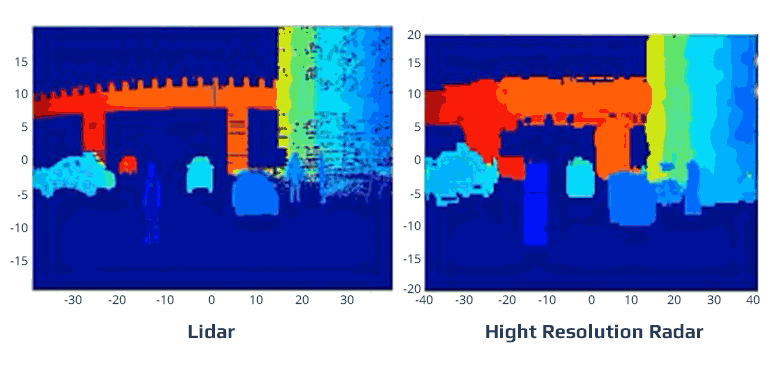
\includegraphics[width=0.5\textwidth]{images/C3_11.png}
    \caption{LiDAR vs high-resolution radar point cloud}
\end{figure}

Compared to the LiDAR, radar point clouds have \textbf{lower accuracy} and a \textbf{worse resolution}.
The reason is the wavelength: LiDARs use lasers with a much shorter wavelength (850--1550\,nm) than the radio waves used by radars (4\,mm at 77\,GHz, 12.5\,mm at 24\,GHz), and this allows them to detect smaller objects.
On the other hand, radars are \textbf{robust} and reliable, they work very well in \textbf{bad weather conditions} (unlike LiDARs) and they are \textbf{cheaper}.
For these reasons the radar is the most used automotive sensor for object detection and tracking, and it is deployed in many commercial vehicles for ADAS features like adaptive cruise control or collision avoidance.

\begin{infobox}[How the distance is computed (FMCW radar)]
\begin{minipage}[c]{0.6\linewidth}
Automotive radars transmit a \textbf{chirp}, a signal whose frequency increases linearly over a sweep bandwidth $F$ during the chirp time $t_c$.
The reflected signal is the same chirp delayed by $t_{echo} = \frac{2R}{c}$, so at any instant the two signals differ by a constant \textbf{beat frequency} $f_b$.
Since the slope of the chirp is $\frac{f_b}{t_{echo}} = \frac{F}{t_c}$, the distance of the target is
\[
R = \frac{c}{2}\,\frac{f_b}{F}\,t_c
\]
\end{minipage}\hfill
\begin{minipage}[c]{0.36\linewidth}
    \centering
    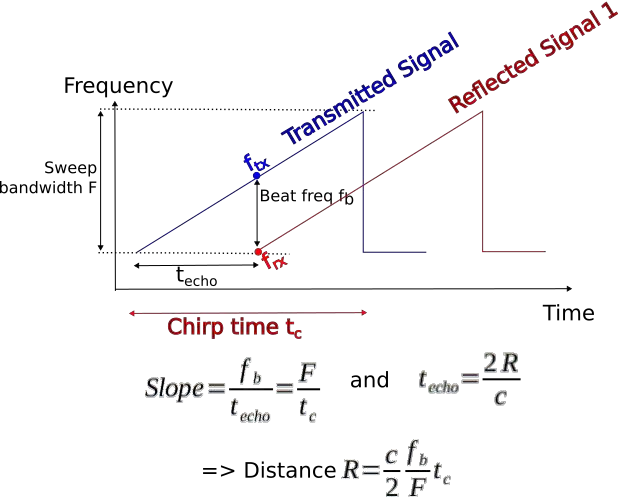
\includegraphics[width=\linewidth]{images/C3_12.png}
\end{minipage}
\end{infobox}

\paragraph{Radar types}
Depending on how much processing is done on board, we distinguish three levels of radar.
A \textbf{low-level radar} outputs the \textbf{raw radar data} (the in-phase and quadrature signals of each range--Doppler cell) and performs no processing on board, so an external unit must interpret the data.
A \textbf{mid-level radar} outputs pre-processed data: a \textbf{point cloud} where each point has \textbf{range, azimuth, elevation and velocity}, but without object tracks or classifications.
A \textbf{high-level radar} provides fully processed data, i.e.\ \textbf{bounding boxes} and \textbf{object tracks}, and it is able to classify the objects and predict their motion.
Obviously, the higher the level, the higher the computational cost on the sensor.

The difference is clear by looking at the messages produced by the three levels:
\begin{lstlisting}[language={}]
// Low-level: raw I/Q signal for each range-Doppler cell
{ "range_bin": 0, "doppler_bin": 1, "I": 0.019, "Q": -0.021 }
// Mid-level: point cloud
{ "range_m": 48.3, "azimuth_deg": -2.1, "elevation_deg": 0.4,
  "radial_velocity_mps": -12.5, "snr_db": 25.0 }
// High-level: tracked and classified objects
{ "track_id": 102, "type": "pedestrian", "position_m": {"x": 20.5, "y": 1.4},
  "velocity_mps": {"x": -1.2, "y": 0.0}, "predicted_path": "crossing" }
\end{lstlisting}

\paragraph{Radar ranges and metrics}
\begin{wrapfigure}{R}{0.36\textwidth}
    \centering
    \vspace{-10pt}
    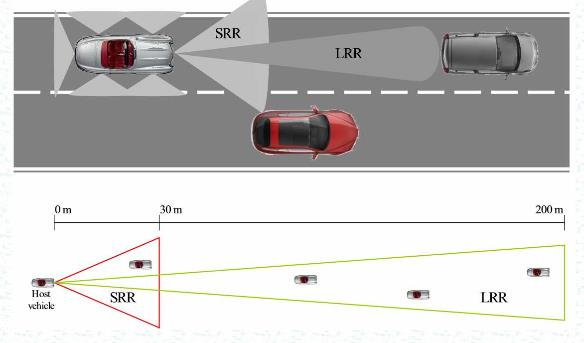
\includegraphics[width=0.35\textwidth]{images/C3_13.png}
    \caption{Short and long range radars}
    \vspace{-10pt}
\end{wrapfigure}
The main metrics of a radar are the \textbf{range}, the \textbf{field of view} and the \textbf{accuracy} in position and speed.
Range and FoV are in a trade-off: a radar with a wide field of view (WFOV) has a short range, while a narrow field of view (NFOV) allows a long range.
For this reason radars are classified by their range:
\begin{compactitemize}
    \item \textbf{SRR} (Short Range Radar), up to $\sim$30\,m: blind spot detection, cross traffic alert, parking;
    \item \textbf{MRR} (Mid Range Radar), up to $\sim$60--100\,m: rear collision warning, automatic emergency braking;
    \item \textbf{LRR} (Long Range Radar), up to $\sim$250\,m: forward collision warning, adaptive cruise control.
\end{compactitemize}

\begin{table}[H]
    \centering
    \begin{tabular}{|l|c|c|c|c|c|}
        \hline
        \textbf{Radar} & \textbf{Frequency (GHz)} & \textbf{Bandwidth} & \textbf{Angle of coverage} & \textbf{Range} & \textbf{Resolution} \\
        \hline
        SRR & 77--81 & 4 GHz & $\pm$20--50° & 0.15--30 m & $\sim$0.1 m \\
        \hline
        MRR & 77--81 & 4 GHz & $\pm$6--10° & 1--100 m & $\sim$0.5 m \\
        \hline
        LRR & 76--77 & 1 GHz & $\pm$5--7.5° & 10--250 m & $\sim$0.5 m \\
        \hline
    \end{tabular}
    \caption{Characteristics of short, mid and long range radars}
\end{table}

\noindent\begin{minipage}[c]{0.6\textwidth}
Summing up, the radar is \textbf{cheap}, small, it \textbf{detects speed} directly and it works well in the dark, in bright light and in \textbf{extreme weather} (snow, fog, rain).
Its main weakness is the \textbf{low resolution}, which makes it hard to classify the objects, and like the LiDAR it does not provide colour information.
This is why radar and LiDAR (or cameras) are often combined with sensor fusion.
\end{minipage}\hfill
\begin{minipage}[c]{0.36\textwidth}
    \centering
    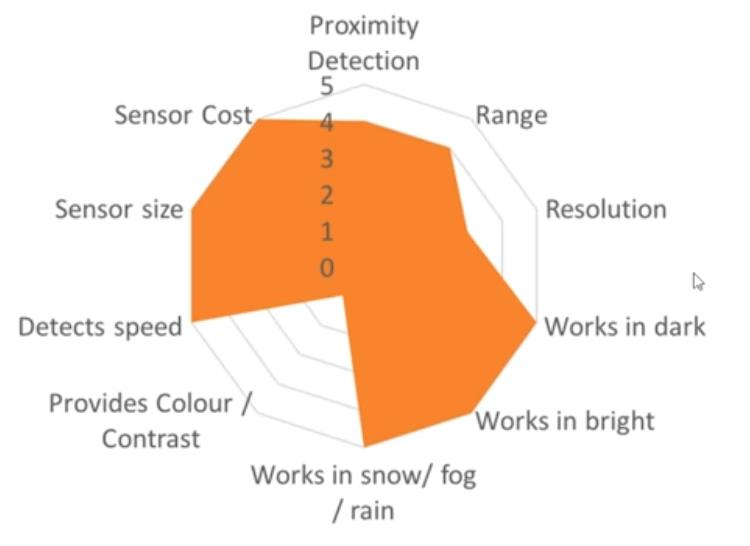
\includegraphics[width=\linewidth]{images/C3_14.png}
    \captionof{figure}{Radar strengths and weaknesses}
\end{minipage}

\subsubsection{Ultrasonic sensor (Sonar)}
\noindent\begin{minipage}[c]{0.6\textwidth}
The \textbf{ultrasonic sensor} is a surround sensor that measures the distance to \textbf{nearby} obstacles using \textbf{ultrasonic sound waves}.
It emits high-frequency sound waves (typically 40--60\,kHz) and, like the other ranging sensors, computes the distance from the time the sound takes to be reflected back.

\vspace{4pt}It has a short range ($\sim$0.2--5\,m), a field of view of about 60--120° and an accuracy of a few centimetres in normal conditions.
\end{minipage}\hfill
\begin{minipage}[c]{0.36\textwidth}
    \centering
    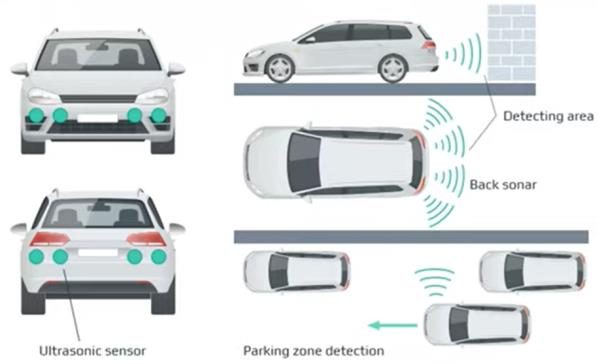
\includegraphics[width=\linewidth]{images/C3_15.png}
    \captionof{figure}{Ultrasonic sensors for parking}
\end{minipage}

Ultrasonic sensors are \textbf{cheap} and, since they use sound instead of light, they are \textbf{not affected by lighting and precipitation}.
However, they become \textbf{unreliable} if the material of the obstacle absorbs the sound, and their short range makes them unsuitable for complex use cases.
For these reasons they are mainly used for \textbf{parking} scenarios (parking sensors, parking assist).

\subsection{Cameras}
Cameras are \textbf{passive} sensors: they do not emit any signal, but capture the light coming from the scene.
They are cheap and provide the richest information (colours, textures, text on signs), which makes them fundamental for recognising \textbf{what} the objects are.
Depending on the number of lenses and on the portion of the spectrum they capture, we have different types of cameras.

\subsubsection{Monocular camera}
\begin{wrapfigure}{R}{0.41\textwidth}
    \centering
    \vspace{-10pt}
    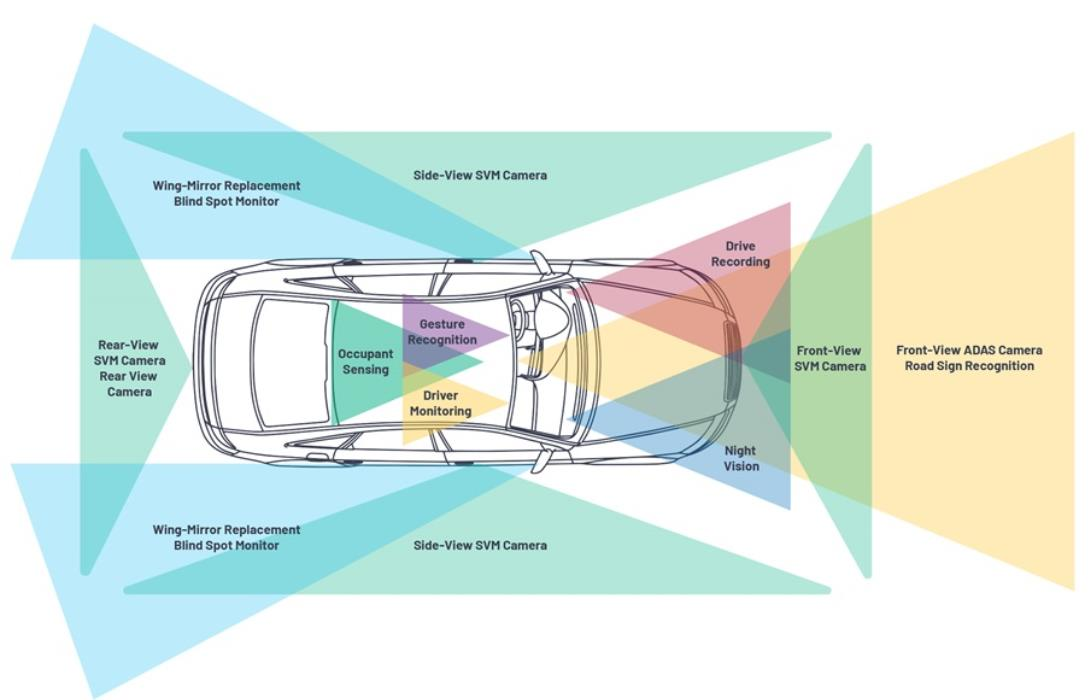
\includegraphics[width=0.4\textwidth]{images/C3_16.png}
    \caption{Cameras around the vehicle and their applications}
    \vspace{-10pt}
\end{wrapfigure}
A \textbf{monocular camera} is a single-lens camera, meaning that it has only \textbf{one optical path} to capture images: the light enters the lens, strikes the sensor and is converted into a digital signal.
They are \textbf{low cost} and give a lot of information, but we lose an important detail: the \textbf{depth}.
There are methods to estimate it from a single image, but very often their error is too high.

Monocular cameras are generally used to \textbf{detect and track objects} (pedestrians, cars) and to detect \textbf{traffic elements} such as lane boundaries, traffic signs and traffic lights, using algorithms like optical flow, Structure from Motion (SfM), image segmentation and classification, feature detection and matching.
Some companies also use omnidirectional cameras to \textbf{localize} the vehicle.
Typical applications are collision warning, lane departure warning, lane keeping assist, lane centering and blind spot detection.
Cameras are especially important for \textbf{collision warning}: from 2028 all new cars will have to implement a collision warning also for pedestrians, and this requires cameras.

The main metrics of a camera are the \textbf{resolution} (number of pixels of the image), the \textbf{field of view} (horizontal and vertical angle visible to the camera), the \textbf{dynamic range}, the \textbf{frame rate} (FPS) and the \textbf{interface} (Ethernet or GMSL).

\paragraph{Resolution and frame rate}
Resolution and frame rate have a direct impact on safety.
A higher \textbf{resolution} gives a \textbf{longer detection range}: a 1\,MP camera detects pedestrians up to about 34\,m (enough for rear-view or basic front cameras), while an 8\,MP camera reaches about 101\,m, as needed in ADAS and AD.
The price is higher computational and power requirements, and worse performance in low-light conditions.

A higher \textbf{frame rate} gives a \textbf{shorter stopping distance}, because the system detects and reacts to the objects faster: at 80\,km/h, a 10\,fps camera leads to a stopping distance of 55\,m (fine for parking assistance), while at 30\,fps it drops to 45\,m (needed for high-speed applications).
Again, this improves latency and tracking but requires more processing power.

In practice, carmakers still integrate \textbf{low-resolution cameras}: they must be resistant to weather, vibrations and hits, and above all \textbf{high-resolution cameras are computationally expensive}.

\begin{figure}[H]
    \centering
    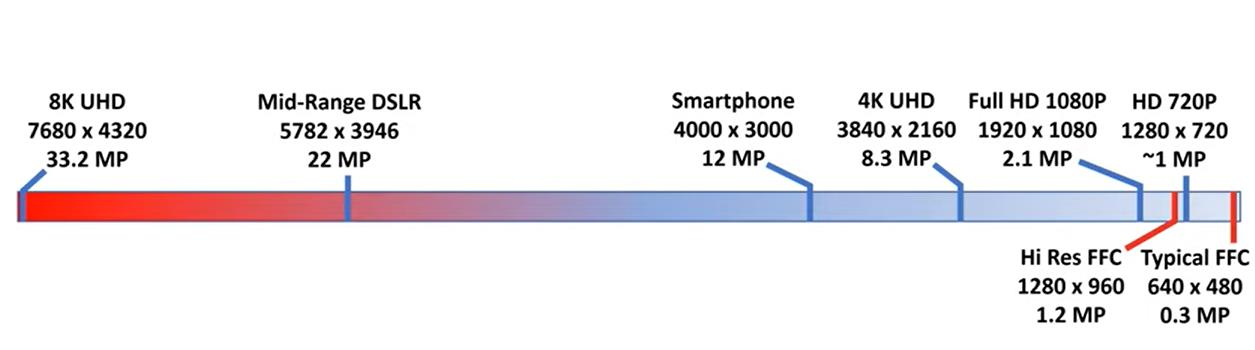
\includegraphics[width=0.7\textwidth]{images/C3_17.png}
    \caption{Resolution of common cameras compared to automotive ones}
\end{figure}

\noindent\begin{minipage}[c]{0.6\textwidth}
Summing up, cameras are cheap, have the highest resolution and provide colour and contrast; they produce a huge amount of data, which is perfect for deep learning, and they are the sensor most similar to what humans use to drive.
On the other hand they are \textbf{bad at depth estimation}, they cannot measure speed directly and they \textbf{do not work well in the dark and in extreme weather}.
\end{minipage}\hfill
\begin{minipage}[c]{0.36\textwidth}
    \centering
    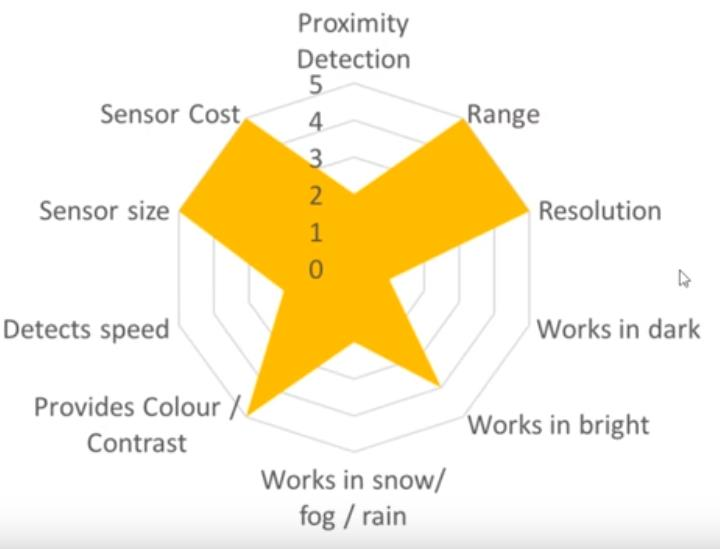
\includegraphics[width=\linewidth]{images/C3_18.png}
    \captionof{figure}{Camera strengths and weaknesses}
\end{minipage}

\begin{infobox}[Sony Vision-S]
A good example of how many sensors a modern vehicle can mount is the Sony Vision-S prototype: 40 sensors in total, of which 18 cameras, 18 radars and 4 LiDARs.
\end{infobox}

\subsubsection{Stereo camera}
\begin{wrapfigure}{R}{0.36\textwidth}
    \centering
    \vspace{-10pt}
    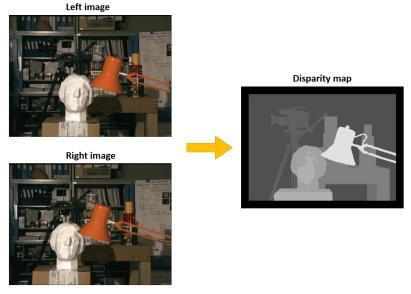
\includegraphics[width=0.35\textwidth]{images/C3_19.png}
    \caption{Disparity map from the left and right images}
    \vspace{-10pt}
\end{wrapfigure}
A \textbf{stereo camera} has \textbf{two or more lenses}, placed at some distance from each other, to simulate the human \textbf{binocular vision}: it captures the scene from slightly different angles, so that we can recover the third dimension.
The distance between the lenses matters: lenses closer together give a better depth estimation at short distances, while lenses farther apart are more effective at greater distances.

The system identifies corresponding features (corners, edges, textures) in the left and right images and compares them to build a \textbf{disparity map}, which encodes for each point the horizontal shift (in pixels) between the two images.
Brighter areas mean a bigger shift, so the object is \textbf{closer}; darker areas mean a smaller shift, so the object is \textbf{farther}.
Using the disparity together with the camera calibration we compute the distance of the objects and generate a \textbf{depth map}, an image where each pixel contains depth information.

Stereo cameras are cheap and give depth, but they are not as precise as LiDARs and radars.

\begin{infobox}[Subaru EyeSight]
Subaru EyeSight is a stereo-camera ADAS used for lane departure warning, forward collision warning, adaptive cruise control and emergency braking, without any radar. Whether it works better than radar-based ADAS systems is still an open question.
\end{infobox}

\subsubsection{Thermal and infrared cameras}
A \textbf{thermographic camera} creates an image using \textbf{infrared radiation}, just like a common camera forms an image using visible light.
Their typical use case is at \textbf{night}: they are used to implement night vision systems, often offered as optional equipment.
We distinguish two types:
\begin{compactitemize}
    \item \textbf{Thermal cameras} detect \textbf{heat} (thermal radiation) instead of visible light, creating images from heat emissions. This makes them ideal for night vision and poor visibility conditions. An example is the LWIR (Long-Wave Infrared) camera, with a wavelength of 8--14\,$\mu$m.
    \item \textbf{Infrared cameras} detect the \textbf{near-infrared} (NIR) light reflected by the objects (0.7--1\,$\mu$m), just beyond the visible spectrum. They are commonly used for proximity sensing, object recognition and \textbf{driver monitoring} (interior sensing).
\end{compactitemize}

\begin{figure}[H]
    \centering
    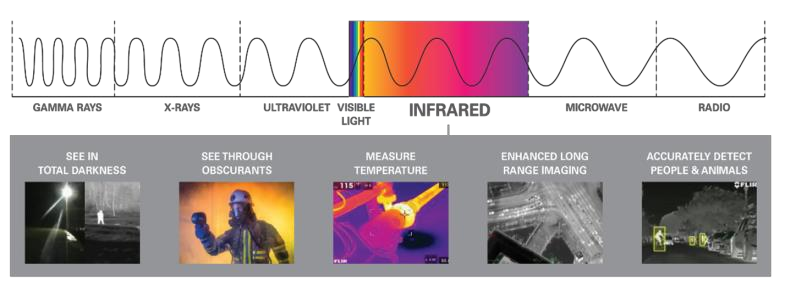
\includegraphics[width=0.6\textwidth]{images/C3_20.png}
    \caption{The same scene captured at different wavelengths}
\end{figure}

\subsubsection{Event-based camera}
\noindent\begin{minipage}[c]{0.55\textwidth}
Our eyes work in a completely different way from today's cameras.
Traditional cameras capture static frames at \textbf{regular intervals} and process them in sequence, so the information between two frames can be lost, especially in fast-moving scenes.

\vspace{4pt}\textbf{Event-based} cameras instead capture only the \textbf{changes in brightness} at each pixel: each pixel reports an \textbf{event} only when it detects a change, so the camera understands \textbf{when something changes} in the scene and responds in real time.
\end{minipage}\hfill
\begin{minipage}[c]{0.41\textwidth}
    \centering
    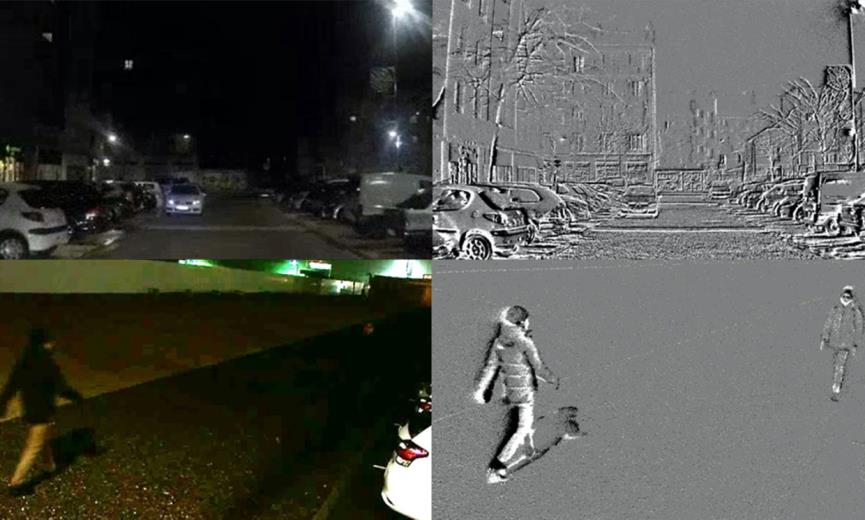
\includegraphics[width=\linewidth]{images/C3_21.png}
    \captionof{figure}{Standard frames vs events}
\end{minipage}

\vspace{6pt}Since they only transmit what changes, event cameras are very \textbf{efficient} in terms of power and computing resources and have a very high dynamic range.
They are starting to be used, mainly on \textbf{drones}.

\subsection{Localization sensors}
The last family of sensors is used to answer the question ``\textit{where is the vehicle?}''.
Some of them are exteroceptive (GPS, which relies on external satellites), others are proprioceptive (IMU and wheel encoders, which only measure the motion of the ego vehicle).
None of them is accurate enough alone, so they are always combined.

\subsubsection{GPS}
\begin{wrapfigure}{R}{0.31\textwidth}
    \centering
    \vspace{-10pt}
    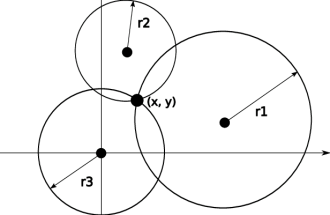
\includegraphics[width=0.3\textwidth]{images/C3_22.png}
    \caption{Trilateration}
    \vspace{-10pt}
\end{wrapfigure}
The \textbf{Global Positioning System} (GPS) is a satellite-based radio navigation system.
Each satellite broadcasts two pieces of information: its \textbf{location} and the \textbf{time}.
The receiver computes its distance from the satellite from the difference between the time the signal was sent and the time it was received ($distance = speed \cdot time$).

A single satellite is not enough: knowing the distance from one satellite only tells us that we are on a sphere around it.
Intersecting the spheres of more satellites we find our position; this technique is called \textbf{trilateration} (it is often called triangulation, but it uses distances, not angles).
In principle three satellites would be enough for $(x, y, z)$, but in practice we need \textbf{four}: the satellites have extremely precise atomic clocks, while the clock of the receiver is not precise at all, and even a tiny time error becomes a big distance error at the speed of light.
So the unknowns are four, $(x, y, z)$ and the \textbf{clock offset} of the receiver, and we need four satellites.

The position returned by a GPS is therefore \textbf{not very precise} (about 15\,m nominal accuracy), and there are many other sources of error:
\begin{compactitemize}
    \item \textbf{Atmospheric effects}: ionospheric and tropospheric delays slow down the signal, causing meter-level errors;
    \item \textbf{Multipath interference}: the signal is reflected by buildings, vehicles or terrain before reaching the receiver;
    \item \textbf{Satellite geometry} (GDOP): a poor distribution of the visible satellites reduces the accuracy;
    \item \textbf{Obstructions}: trees, tunnels, urban canyons or indoor environments block or degrade the signal.
\end{compactitemize}
To solve these problems there are several variants of GPS, such as DGPS, RTK and PPP.

\paragraph{DGPS}
\begin{wrapfigure}{R}{0.41\textwidth}
    \centering
    \vspace{-10pt}
    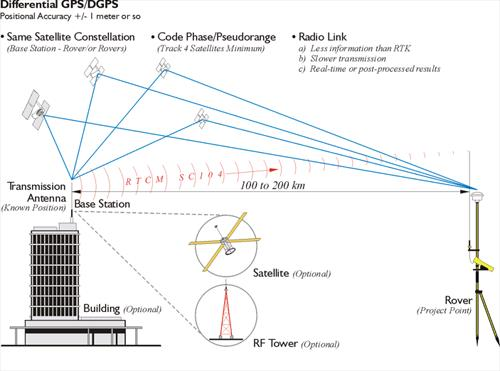
\includegraphics[width=0.4\textwidth]{images/C3_23.png}
    \caption{Differential GPS}
    \vspace{-10pt}
\end{wrapfigure}
The \textbf{Differential GPS} (DGPS) is based on the concept of \textbf{base station}.
A network of fixed \textbf{reference stations} is installed at locations with precisely known coordinates.
Each station compares its true position with the one computed from the satellites, and obtains the real-time correction (the \textbf{differential error}).
These corrections are broadcast to the mobile receivers (\textbf{rovers}), which apply them to their own GPS measurements to obtain a more accurate position.
In other words, when the vehicle localizes itself, it uses both the satellites and the base stations.

The distance from the base station matters: the closer the rover is to the reference station, the more similar the errors they see, and the smaller the residual atmospheric and satellite errors.
With the best implementations we go from the 15\,m of the nominal GPS to about 1--3\,cm.

\paragraph{GPS RTK}
\noindent\begin{minipage}[c]{0.6\textwidth}
\textbf{Real Time Kinematic} (RTK) is a form of DGPS that uses new techniques to further enhance the precision.
A base station (fixed, or even portable) knows its exact position and receives the same satellite signals as the rover.
It computes the \textbf{carrier-phase correction}, i.e.\ the precise error in the satellite signals, and sends it to the rover, which applies it to its own measurements to get an instant and highly accurate position.
\end{minipage}\hfill
\begin{minipage}[c]{0.36\textwidth}
    \centering
    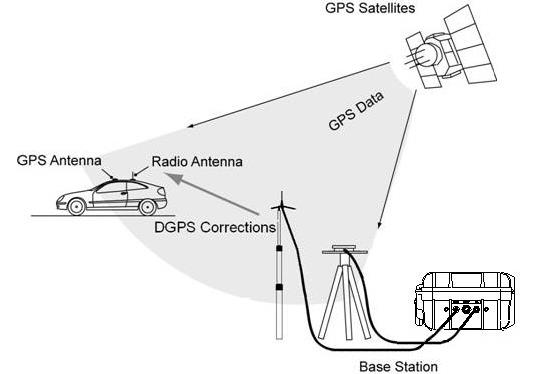
\includegraphics[width=\linewidth]{images/C3_24.png}
    \captionof{figure}{GPS RTK}
\end{minipage}

\vspace{6pt}The main advantage is that RTK \textbf{solves the ionospheric and tropospheric delays} still present in DGPS, i.e.\ the errors caused by the radio waves slowing down while crossing the ionized layer of the atmosphere (ionosphere) and its moisture-rich lower layer (troposphere).
Because of its precision, RTK is mostly used to \textbf{test and verify} the localization performance of ADAS systems (benchmarking).

\subsubsection{IMU}
\noindent\begin{minipage}[c]{0.6\textwidth}
The \textbf{Inertial Measurement Unit} (IMU) measures the \textbf{acceleration}, the \textbf{angular rate} and the \textbf{orientation} of the vehicle, using a combination of \textbf{accelerometers}, \textbf{gyroscopes} and \textbf{magnetometers}.
It returns the linear acceleration (accelerometers), the angular velocity (gyroscopes) and the magnetic field (magnetometers).
Combining them we obtain the orientation: accelerometers give roll and pitch, gyroscopes improve them and add the yaw, and magnetometers further improve the yaw.
\end{minipage}\hfill
\begin{minipage}[c]{0.36\textwidth}
    \centering
    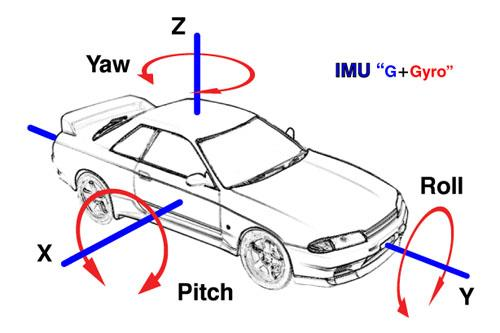
\includegraphics[width=\linewidth]{images/C3_25.png}
    \captionof{figure}{Roll, pitch and yaw}
\end{minipage}

\paragraph{INS and the drift problem}
The IMU alone only tells us how the vehicle is moving. An \textbf{Inertial Navigation System} (INS) is the navigation system built on top of an IMU: it uses its measurements to continuously estimate the \textbf{position}, \textbf{velocity} and \textbf{orientation} of the vehicle.
It performs \textbf{dead reckoning}: starting from a known position, it integrates speed and heading over time to track the movement, without any external signal.

\begin{wrapfigure}{R}{0.31\textwidth}
    \centering
    \vspace{-10pt}
    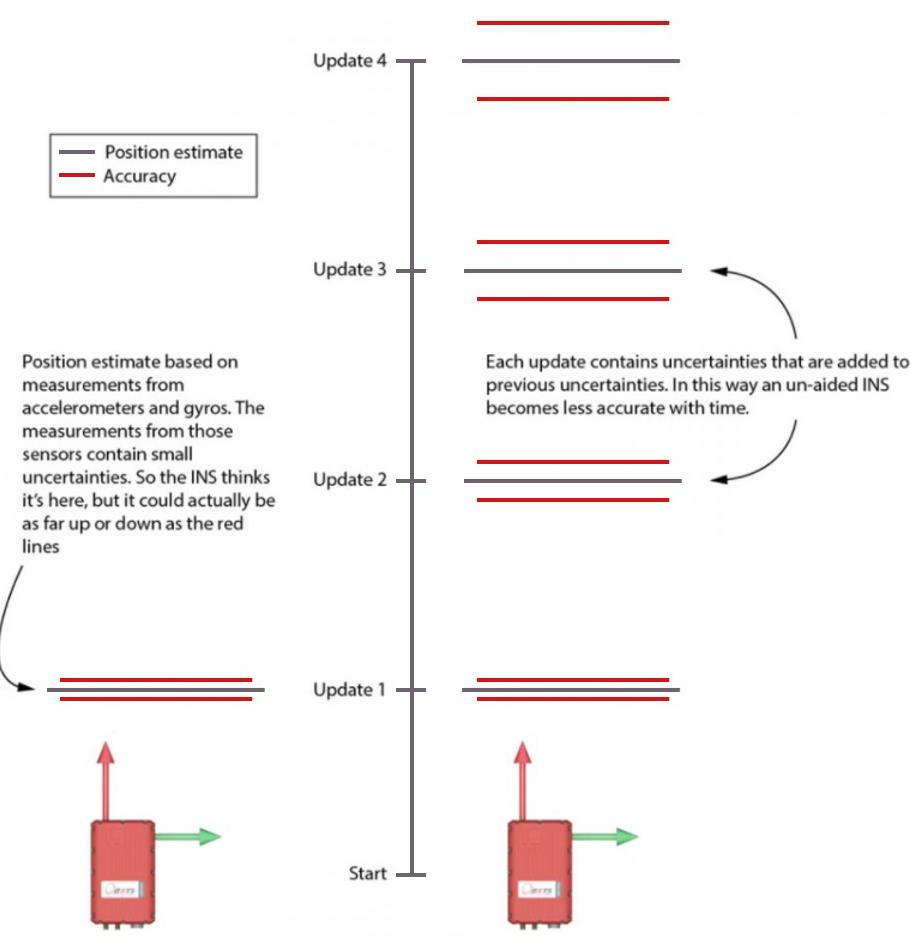
\includegraphics[width=0.3\textwidth]{images/C3_26.png}
    \caption{INS drift: the uncertainty grows at every update}
    \vspace{-10pt}
\end{wrapfigure}
The problem of this approach is the \textbf{drift}, i.e.\ the accumulation of small errors in the accelerometer and gyroscope measurements, which gradually makes the position estimate inaccurate.
Every time we read a sensor there is a minuscule error: this is not a problem if we read the data only once, but the INS continuously integrates the acceleration to obtain velocity and position, so every error, however small, is \textbf{accumulated over time}.
For example, if a sensor gives the position with 1\,cm of error and we keep building on its previous readings, after $n$ measurements the error can grow up to $n$\,cm.

For this reason an INS always needs an \textbf{external reference}, such as the GPS, to periodically correct the drift.

\subsubsection{Wheel odometry}
\noindent\begin{minipage}[c]{0.6\textwidth}
\textbf{Wheel odometry} estimates the position, orientation and speed of the vehicle by measuring \textbf{how much the wheels rotate} over time, using wheel encoders (sensors that count the wheel revolutions).
The encoders measure the angular displacement of each wheel; knowing the wheel radius and the vehicle geometry, the system converts the rotations into a linear distance and a yaw (heading) change, and integrates these increments to update the pose $(x, y, \theta)$ of the vehicle.
\end{minipage}\hfill
\begin{minipage}[c]{0.36\textwidth}
    \centering
    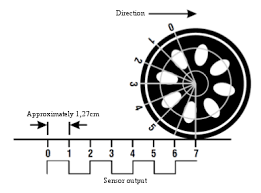
\includegraphics[width=\linewidth]{images/C3_27.png}
    \captionof{figure}{Wheel encoder}
\end{minipage}

\vspace{6pt}Like the INS, wheel odometry suffers from \textbf{drift}: wheel slip, uneven terrain or encoder noise cause cumulative errors, and the accuracy degrades with the distance unless it is corrected with absolute sensors.
This is why, in general, wheel odometry, GPS, IMU (and LiDAR) are \textbf{used together} to correct the localization of the vehicle.

\subsection{Comparison and sensor fusion}
After analysing all the sensors, the main conclusion is that \textbf{no single sensor can provide accurate information in all conditions}.
For instance, cameras perform poorly when the weather is not favourable (night or rain); radar, unlike cameras, works well in poor weather, but its resolution is not good enough to classify the objects; LiDAR is accurate in 3D, but it is expensive and it suffers in fog and cannot read signs or see colours.

\begin{table}[H]
    \centering
    \begin{tabular}{|l|c|c|c|c|}
        \hline
        \textbf{Performance aspect} & \textbf{Human} & \textbf{Radar} & \textbf{LiDAR} & \textbf{Camera} \\
        \hline
        Object detection              & Good & Good & Good & Fair \\
        \hline
        Object classification         & Good & Poor & Fair & Good \\
        \hline
        Distance estimation           & Fair & Good & Good & Fair \\
        \hline
        Edge detection                & Good & Poor & Good & Good \\
        \hline
        Lane tracking                 & Good & Poor & Poor & Good \\
        \hline
        Visibility range              & Good & Good & Fair & Fair \\
        \hline
        Poor weather performance      & Fair & Good & Fair & Poor \\
        \hline
        Dark or low illumination      & Poor & Good & Good & Fair \\
        \hline
    \end{tabular}
    \caption{Sensing capabilities of human drivers and of the AV sensors}
\end{table}

Moreover, each sensor generates a \textbf{different amount of raw data}: from tens of KB per second for radar, sonar and GPS, up to tens of MB per second for cameras and LiDARs.
For all these reasons, the AV software stack is normally built \textbf{combining different sensors}, which allows to obtain a better representation of the environment.

\begin{figure}[H]
    \centering
    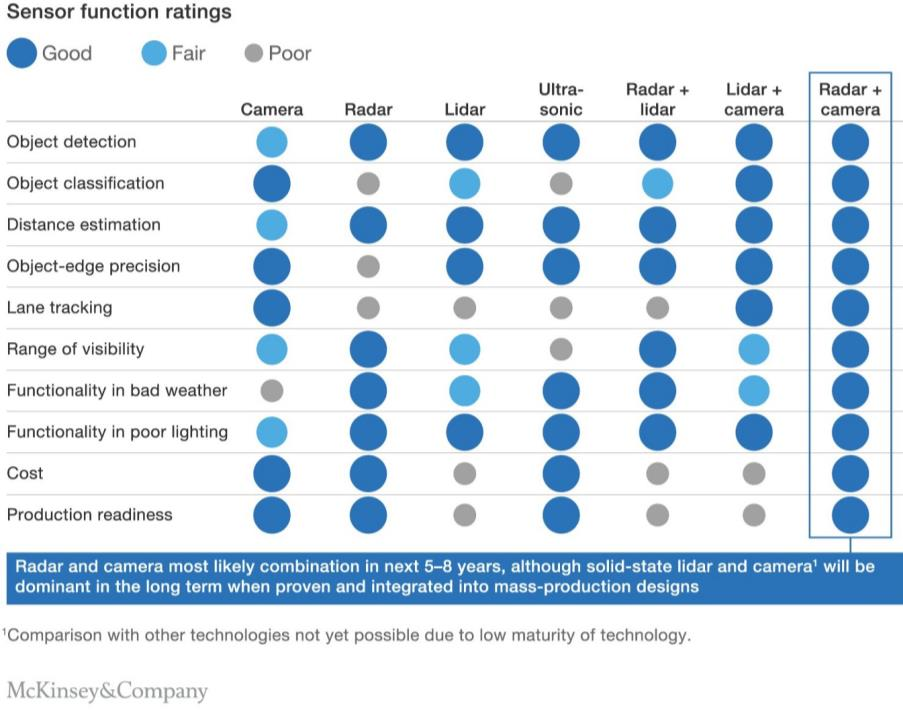
\includegraphics[width=0.65\textwidth]{images/C3_28.png}
    \caption{Sensor function ratings, alone and combined}
\end{figure}

The figure above also shows which combinations are expected in the market: \textbf{radar + camera} is the most likely combination in the next years, since it is good in every aspect, cheap and production-ready, while solid-state LiDAR + camera is expected to become dominant in the long term, once proven and integrated into mass-production designs.

\subsubsection{Sensor fusion}
\noindent\begin{minipage}[c]{0.55\textwidth}
To overcome the limitations of the single sensors, \textbf{sensor fusion} can be applied (``unity makes strength''): the data of different sensors are combined so that the strengths of one compensate for the weaknesses of the others.

\vspace{4pt}Sensor fusion also provides \textbf{redundancy} for self-driving vehicles: if one sensor fails or is blinded, the others can still perceive the environment.
For instance, LiDAR and radar data can be fused to obtain an improved 3D object detection, independently of the weather conditions.
\end{minipage}\hfill
\begin{minipage}[c]{0.41\textwidth}
    \centering
    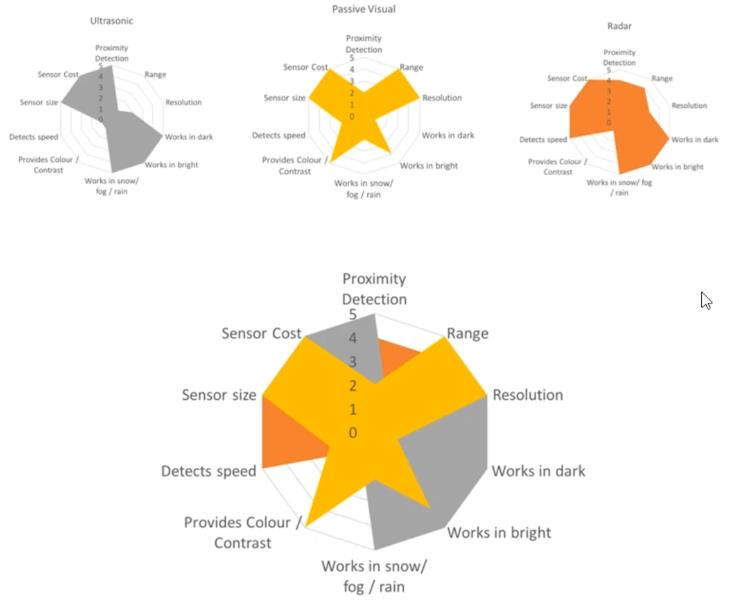
\includegraphics[width=\linewidth]{images/C3_29.png}
    \captionof{figure}{Ultrasonic, camera and radar combined cover each other's weaknesses}
\end{minipage}

\vspace{6pt}In this course we will use sensor fusion (\textbf{radar + LiDAR}) to improve the \textbf{localization} system of the car.
